\section{Usar complementos}\index{plugins}

\subsection{Una introducción al uso de complementos}\label{label_introplugin}

QGIS se ha diseñado con una arquitectura de complementos. Esto permite que se añadan nuevas funciones a la aplicación. Muchas de las funciones actuales de QGIS están en realidad implementadas como complementos.

Hay dos tipos de complementos en QGIS: integrados o aportados por usuarios. \index{plugins!types} Un complemento integrado es mantenido por el equipo de desarrollo de QGIS y forma parte de cada distribución de QGIS. Un complemento aportado por usuarios es un complemento externo que es mantenido por el autor individual. La web del SVN de QGIS (\url{http://svn.qgis.org}) sirve algunos complementos aportados por usuarios.

\subsubsection{Encontrar e instalar un complemento}
Cuando instala QGIS, todos los complementos integrados están incluidos (vea el capítulo \ref{sec:core_plugins}). \index{plugins!installing}
% Additional user-contributed
% plugins may be available on the QGIS Community site. To see what
% user-contributed plugins are available, see the plugins page on the Community
% site (\url{http://community.qgis.org/plugins}).\index{plugins!user
% contributed}

De forma típica, los complementos aportado por usuarios se distribuyen en forma de código fuente y hay que compilarlos. Para instrucciones sobre la compilación e instalación de un complemento aportado por usuarios, vea la documentación incluida con el complemento.

\subsubsection{Administrar complementos}\label{sec:managing_plugins}
\index{plugins!managing} La administración de complementos consiste en cargarlos o descargarlos desdes QGIS. Los complementos cargados se «recuerdan» cuando sale de la aplicación y son restaurados la siguiente vez que ejecuta  QGIS.

Para administrar complementos, abra el \textsl{Administrador de complementos} desde el menú \textsl{Complementos}. \index{plugins!manager}El Administrador de complementos muestra todos los complementos disponibles y su estado (cargados o no cargados). La Figura \ref{fig:pluginmanager} muestra el diálogo del Administrador de complementos.

\begin{figure}[ht]
   \begin{center}
   \caption{Administador de complementos}\label{fig:pluginmanager}\smallskip
   \includegraphics[clip=true, width=14cm]{pluginmanager2}
\end{center}  
\end{figure}

De forma típica todos los complementos de QGIS se instalan en la misma ubicación. Esta localización se muestra en el campo de texto Directorio de complementos. Le puede decir a QGIS que cargue complementos desde otra localización especificando un directorio distinto.

\begin{Tip}\caption{\textsc{Complementos que se cuelgan}}\index{crashes}
\qgistip{Si nota que QGIS se cuelga al iniciar, puede que haya un complemento que está dando problemas. Puede detener todos los complementos para que no se carguen editando su archivo de configuración guardado (vea \ref{subsec:gui_options} para su localización). Localice la configuración de los complementos y cambie todos los valores a false para evitar que se carguen. Por ejemplo, para evitar que se cargue el complemento Texto delimitado, la entrada en \$HOME/.config/QuantumGIS/qgis.conf en Linux debería ser como esta::\ttfamily{Add Delimited Text Layer=false}.\normalfont Haga esto con cada  complemento en la sección [Plugins]. Luego puede arrancar QGIS y añadir los complementos de uno en uno desde el Administrador de complementos para determinar cuál está ocasionando los problemas.
}
\end{Tip} 

\subsubsection{Proveedores de datos}\index{data providers}

Los proveedores de datos son complementos «especiales» que proporcionan acceso a un almacén de datos. De forma predeterminada, QGIS soporta capas PostGIS y almacenes de datos basados en disco soportados por la biblioteca GDAL/OGR (Apéndice \ref{appdx_ogr}). Un complemento de proveedor de datos amplía la capacidad de QGIS para usar otras fuentes de datos.

Los complementos de proveedores de datos son registrados automáticamente por QGIS al iniciarse. No son gestionados por el Administrador de complementos, pero se usan sin notarlo cuando el tipo de datos correspondiente se añade como capa en QGIS.

\subsubsection{Complementos integrados}\label{sec:core_plugins}\index{plugins!core}

Actualmente QGIS contiene 9 complementos integrados que se pueden cargar usando el Administrador de complementos. La tabla \ref{tab:core_plugins} lista cada uno de los complementos integrados junto con una descripción de su propósito y el icono de la barra de herramientas. Note que el complemento de GRASS no está incluido abajo, porque éste instala su propia barra de herramientas (vea la sección \ref{sec:grass} para ver en detalle las funciones disponibles en el complemento de GRASS).

% minipage is needed to appear the footnote under the table
% SH
\begin{minipage}{\textwidth}
\begin{table}[H]
\centering
\caption{Complementos integrados de QGIS}\label{tab:core_plugins}\medskip
\small
 \begin{tabular}{|l|l|p{4in}|}
\hline \textbf{Icono} & \textbf{Complemento} & \textbf{Descripción} \\
\hline 
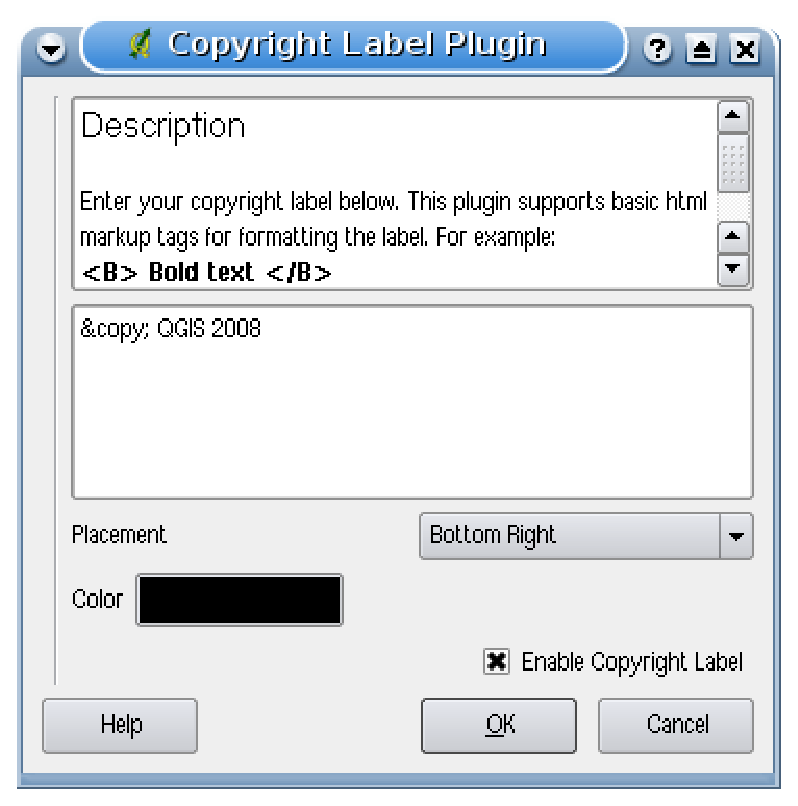
\includegraphics[width=0.7cm]{copyright} & Etiqueta de Copyright \index{plugins!copyright}& Muestra una etiqueta de copyright sobre el lienzo del mapa\\
\hline 
\includegraphics[width=0.7cm]{delim_text} & Texto delimitado \index{plugins!delimited text}& Carga una archivo de texto delimitado que contenga coordenadas X e Y como una capa de puntos \\
\hline 
\includegraphics[width=0.7cm]{gps} & Herramientas de GPS \index{plugins!gps}& Carga y muestra datos de GPS \\
\hline 
\includegraphics[width=0.7cm]{gridmaker} & Creador de cuadrículas \index{plugins!graticule}& Crea una cuadrícula latitud/longitud y la guarda como archivo shape\\
\hline 
\includegraphics[width=0.7cm]{scalebar} & Barra de escala \index{plugins!scalebar}& Añade una barra de escala a la vista del mapa\\
\hline 
\includegraphics[width=0.7cm]{northarrow}& Flecha de Norte \index{plugins!north arrow}& Añada una flecha de Norte a la vista del mapa\\
\hline 
\includegraphics[width=0.7cm]{buffer} & Geoprocesamiento PostgreSQL \index{plugins!geoprocessing}& Crea un área de influencia de una capa PostGIS \\
\hline 

\includegraphics[width=0.7cm]{spiticon} & SPIT \index{plugins!SPIT}& Herramienta de importación de archivos Shape a PostGIS - importa archivos shape a PostgreSQL\\
\hline

\includegraphics[width=0.7cm]{georeferencer} & Georreferenciador\footnote{El complemento Georreferenciador sólo está disponible si tiene instaladas las bibiotecas y cabeceras de gsl durante la compilación. Por favor, revise el capítulo de instalación \ref{sec:install_gsl} para más detalles.} \index{plugin!Georeferencer} & Georreferenciar capas ráster \\
\hline
\includegraphics[width=0.7cm]{wfs-icon} & WFS & Carga y muestra capas WFS \\
\hline
\end{tabular}
\end{table}
\end{minipage}

\normalsize


\begin{Tip}\caption{\textsc{Configuración de complementos guardada en proyectos}}\index{plugins
settings}
\qgistip{Cuando guarda un proyecto .qgs, cualquier cambio que haya hecho en los complementos flecha de Norte, barra de escala y etiqueta de copyright se guardará en el proyecto y se restaurará la próxima vez que cargue el proyecto.
}
\end{Tip}

%
% External Plugins
%
\subsubsection{Complementos externos}\label{sec:external_plugins}\index{plugins!external}

QGIS también viene con algunos complementos desarrollados de forma externa. Éstos no están incluidos con la distribución predeterminada. Sin embargo, se pueden compilar y usar en QGIS.

Actualmente los complementos externos sólo están disponibles directamente desde SVN. Para comprobar todos los complementos externos disponibles haga lo siguiente:
\begin{verbatim}
svn co https://svn.osgeo.org/qgis/trunk/external_plugins external_qgis_plugins
\end{verbatim}

Esto creará la carpeta \texttt{external\_qgis\_plugins} en su carpeta actual. Cada subdirectorio tiene sus propias instrucciones de compilación e instalación. Léalas detenidamente para instalar el complemento.

%
% Plugin template
%
\subsubsection{Plantillas de complementos}\label{sec:plugin_template}\index{plugins!template}

Si quiere desarrollar su propio complemento de QGIS las fuentes principales incluyen un buen script que le guía a través del proceso de crear su propia estructura de directorios de plantillas dentro del árbol de las fuentes de QGIS. El script se encuentra en \texttt{QGIS/src/plugins/plugin\_builder.pl}.

Lo único que hay que hacer es poner el código de sus funciones dentro del complemento (y por supuesto aportar su complemento al equipo de desarrollo de QGIS).

Además de esto, el wiki de QGIS (\url{http://wiki.qgis.org}) y el blog de QGIS (\url{http://blog.qgis.org}) también proporcionan artículos útiles sobre la escritura de su propio complemento. ¡Visite las páginas web para detalles!
